% !TeX root = Bericht_main.tex

\subsection{Aufgabe 31}

In Aufgabe 31 versuchen wir Schritt für Schritt eine sinnvolle Wahl für die Feinheit von Orts- bzw. Zeitdiskretisierung herauszufinden. Dazu ermitteln wir abhängig vom Verfeinerungslevel $level = 0,1,2$ eine sinnvolle Zeitschrittweite, sodass der Fehler der Zeitdiskretisierung kleiner als der Ortsfehler ist und der Startwert des Newton-Verfahrens so gut ist, dass die Newton-Konvergenz quadratisch ist. 
Wir vergleichen dazu die Masse der Konzentration in einem Plot für das exponentielle Wachstum mit $ Reaction = 2.5 $

\begin{figure}[H]
	\centering
	\captionabove{Vergleich der Masse für unterschiedliche Zeitdiskretisierungen}
	\subfigure[auf Level = 0]{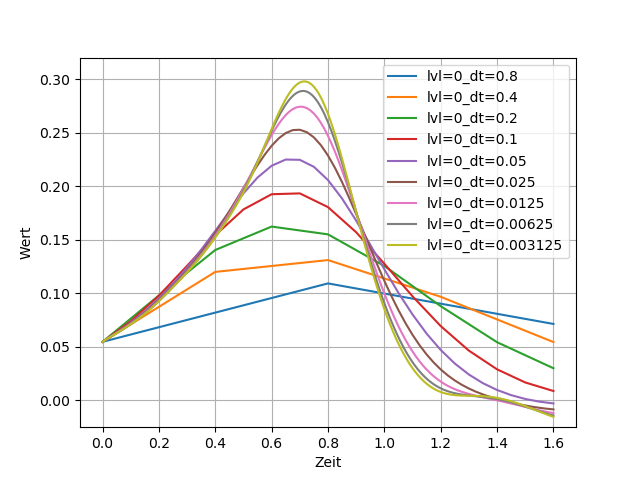
\includegraphics[width=0.85\textwidth]{../Aufgabe31/Maxdiff/zeitvergleich_lvl=0_plot.png}}
\end{figure}
\begin{figure}[H]
	\centering
	\subfigure[auf Level = 1]{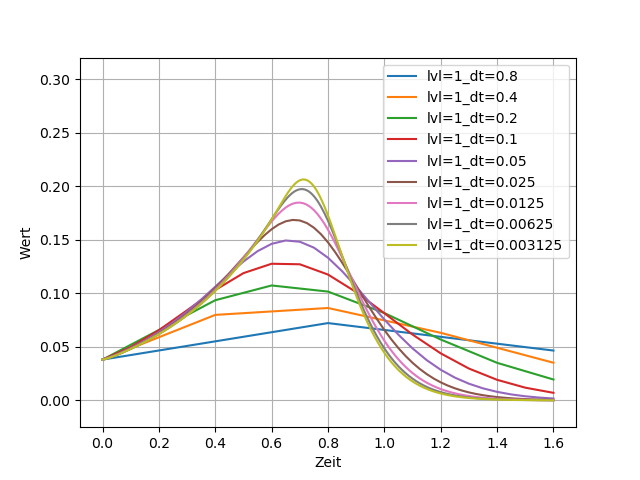
\includegraphics[width=0.85\textwidth]{../Aufgabe31/Maxdiff/zeitvergleich_lvl=1_plot.png}}
\end{figure}
\begin{figure}[H]
	\centering
	\subfigure[auf Level = 2]{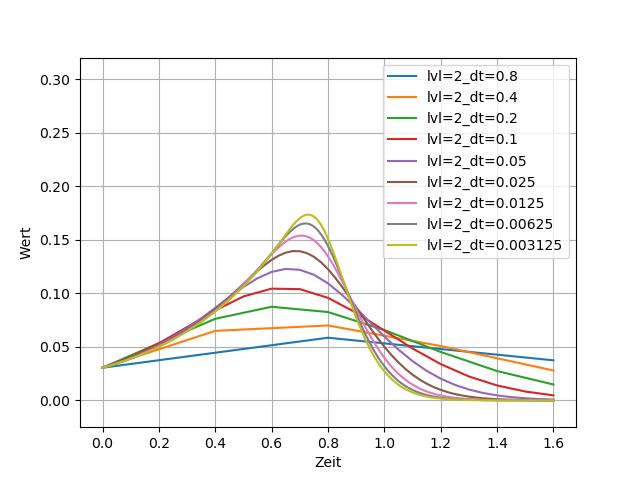
\includegraphics[width=0.85\textwidth]{../Aufgabe31/Maxdiff/zeitvergleich_lvl=2_plot.png}}
\end{figure}

Um zusätzlich zum Fehler der Zeitdiskretisierung auch den Fehler der Ortsdiskretisierung abschätzen zu können, ist es zudem hilfreich auch die verschiedenen Masseplots für eine fest gewählte Zeitdiskretisierung auf den unterschiedlichen Levels zu vergleichen:
 
 \begin{figure}[H]
 	\centering
 	\captionabove{Vergleich der Masse für $Level = 1,2,3$}
 	\subfigure[mit $dt = 0.8$]{\includegraphics[width=0.32\textwidth]{../Aufgabe31/Maxdiff/2vergleich_dt=08_plot.png}}
 	\subfigure[mit $dt = 0.4$]{\includegraphics[width=0.32\textwidth]{../Aufgabe31/Maxdiff/2vergleich_dt=04_plot.png}}
 	\subfigure[mit $dt = 0.2$]{\includegraphics[width=0.32\textwidth]{../Aufgabe31/Maxdiff/2vergleich_dt=02_plot.png}}
 	\subfigure[mit $dt = 0.1$]{\includegraphics[width=0.32\textwidth]{../Aufgabe31/Maxdiff/2vergleich_dt=01_plot.png}}
 	\subfigure[mit $dt = 0.05$]{\includegraphics[width=0.32\textwidth]{../Aufgabe31/Maxdiff/2vergleich_dt=005_plot.png}}
 	\subfigure[mit $dt = 0.025$]{\includegraphics[width=0.32\textwidth]{../Aufgabe31/Maxdiff/2vergleich_dt=0025_plot.png}}
 	\subfigure[mit $dt = 0.0125$]{\includegraphics[width=0.32\textwidth]{../Aufgabe31/Maxdiff/2vergleich_dt=00125_plot.png}}
 	\subfigure[mit $dt = 0.00625$]{\includegraphics[width=0.32\textwidth]{../Aufgabe31/Maxdiff/2vergleich_dt=000625_plot.png}}
 \end{figure}